\documentclass[a4paper,11pt,exos]{nsi} % COMPILE WITH DRAFT


%\pagestyle{empty}
\begin{document}

\setlength{\columnseprule}{0pt}
\setlength{\columnsep}{1cm}

\classe{\premiere spe}
\titre{Variables aléatoires}
\maketitle

\subsection*{Variables aléatoires réelles}

\exo{}
On lance un dé tétraédrique équilibré dont les faces sont numérotées de 1 à 4. Dans chaque cas, déterminer :
\begin{enumerate}[label=\textbullet]
	\item 	Les valeurs prises par la variable aléatoire $X$ ;
	\item 	la loi de probabilité de $X$.	
\end{enumerate}
\begin{enumerate}
	\item 	$X$ est la variable aléatoire qui associe à chaque lancer le double du nombre obtenu.
	\item 	$X$ est la variable aléatoire qui associe à chaque lancer $(-1)^n$ où $n$ est le nombre obtenu.	
\end{enumerate}
%\vspace{0.5cm}


\exo{}
Une urne contient cinq boules indiscernables au toucher numérotées de 1 à 5. On en tire trois simultanément. Soit $M$ la variable aléatoire qui associe au tirage de trois boules le plus petit nombre inscrit sur celles-ci.
\begin{enumerate}
	\item 	Quelles sont les valeurs prises par $M$ ?
	\item 	Déterminer la loi de probabilité de $M$.	
\end{enumerate}
%\vspace{0.5cm}


\exo{}
\begin{minipage}{12cm}
	Une urne contient des jetons, indiscernables au toucher, représentés ci-contre.
	\begin{enumerate}
		\item 	Soit $X$ la variable aléatoire qui associe, au tirage d'un jeton dans l'urne, la valeur du nombre inscrit sur celui-ci.\\
		Déterminer la loi de probabilité de $X$.
	\end{enumerate}
\end{minipage}
\hspace{0.4cm}
\begin{minipage}{5cm}
	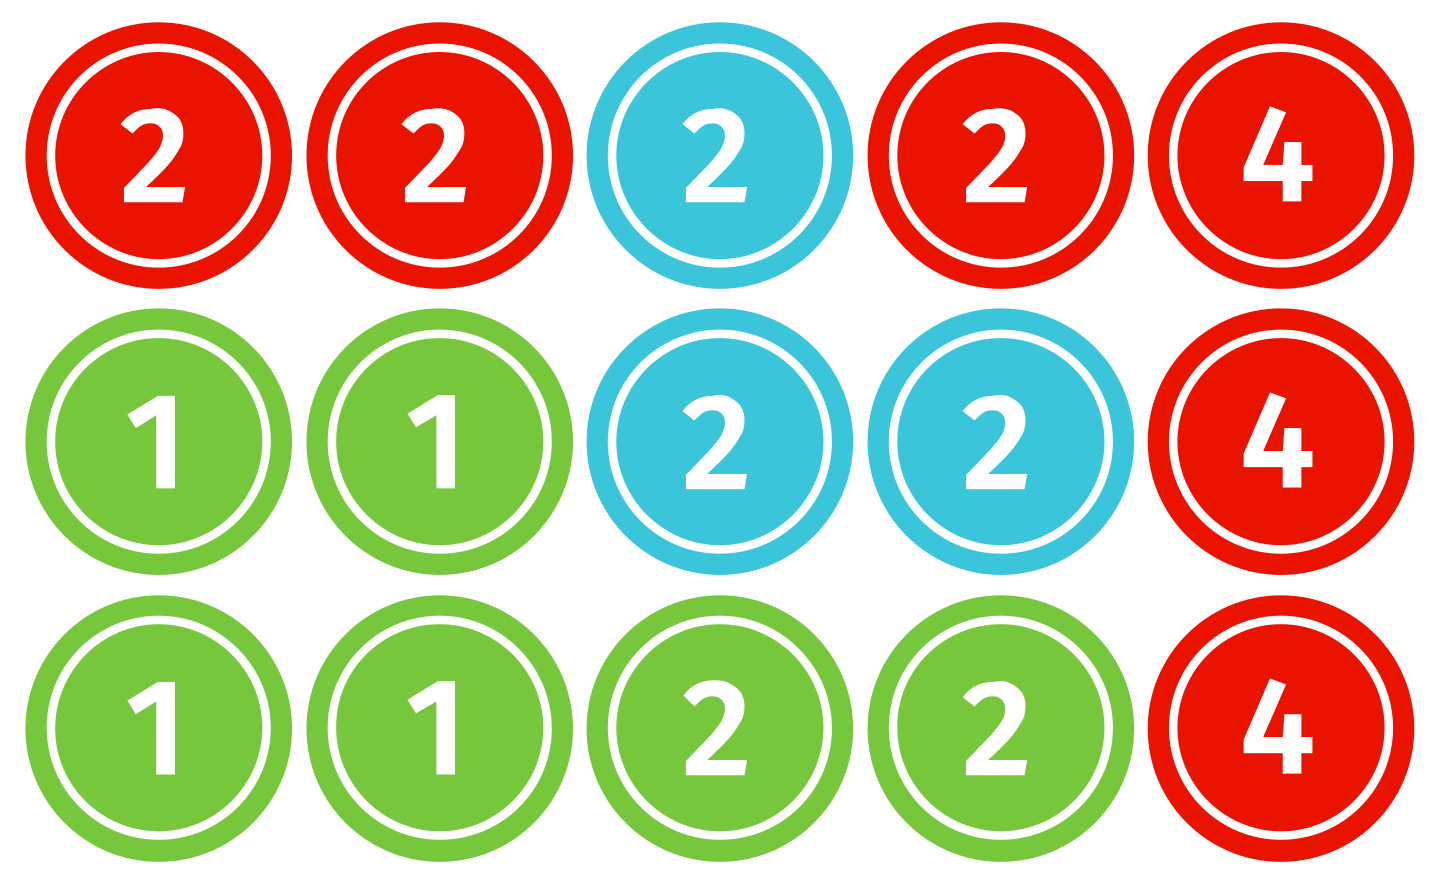
\includegraphics[width=5cm]{jetons}
\end{minipage}
\begin{enumerate}[label=\bfseries 2.]
	\item 	On suppose maintenant que les jetons verts comptent double, les jetons rouges comptent pour moitié	et les jetons bleus sont sans effet.\\
	Soit $Y$ la variable aléatoire qui associe, au tirage d'un jeton dans l'urne, la valeur du nombre inscrit sur celui-ci en tenant compte des modifications.\\
	Déterminer la loi de probabilité de $Y$.
\end{enumerate}
%\vspace{0.5cm}


\exo{}
\begin{minipage}{9cm}
	On étudie le comportement d'une souris dans le labyrinthe ci-contre.\\
	À chaque intersection, la souris choisit au hasard et de manière équiprobable une direction. Soit $X$ la variable aléatoire qui donne le nombre de fromages que la souris a mangés en traversant le labyrinthe.\\
	Déterminer la loi de probabilité de $X$.
\end{minipage}
\begin{minipage}{8.4cm}
	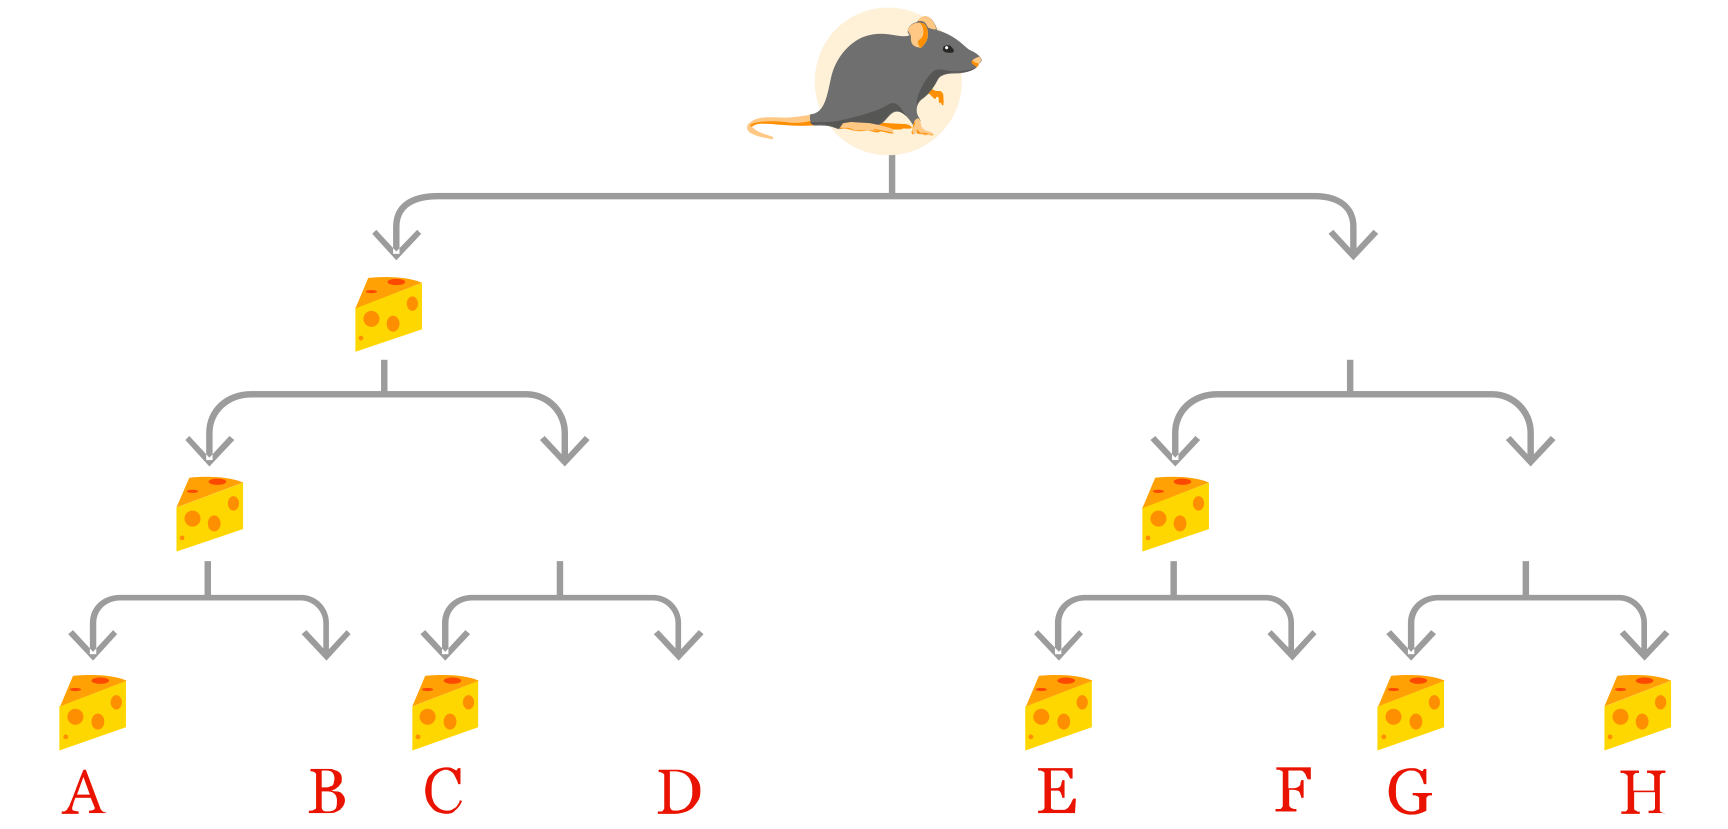
\includegraphics[width=8.4cm]{souris}
\end{minipage}

\vspace{0.5cm}

\begin{minipage}{8.4cm}
	\exo{}
	Une biscuiterie fabrique des cookies qu'elle conditionne en sachets. Les cookies peuvent être aux pépites de chocolat au lait, de chocolat noir ou de chocolat blanc et peuvent contenir ou non des éclats de noisettes.\\
	Pour déterminer le prix $P$ d'un sachet de cookies, la biscuiterie utilise l'algorithme ci-contre :
	\begin{enumerate}
		\item 	Déterminer le prix à payer pour un sachet de différentes variétés de cookies.
		\item 	Les six types de cookies ont exactement la même probabilité d'être produits.\\
		On appelle $X$ la variable aléatoire qui associe à un sachet de cookies son prix de vente.\\
		Déterminer la loi de probabilité de $X$.	
	\end{enumerate}
	
\end{minipage}
\hspace{0.5cm}
\begin{minipage}{8.5cm}
    \begin{encadrecolore}{Algorithme}{UGLiBlue}
P <- 2,5\\
Si les cookies sont aux pépites de chocolat noir :\\
\hspace*{1em}  P <- P+1\\
Sinon :\\
\hspace*{1em}   Si les cookies sont aux pépites de chocolat blanc :\\
\hspace*{2em}      P <- P+0,5\\
\hspace*{1em}   Fin Si\\
Fin Si\\
Si les cookies ont des éclats de noisettes :\\
\hspace*{1em}   P <- P+0,5\\
Fin Si
	\end{encadrecolore}
\end{minipage}

\vspace{1cm}



\begin{minipage}{10.9cm}
	\exo{ La planche de Galton}
	Un joueur lâche une bille sur une planche inclinée sur laquelle sont plantés des clous comme sur la figure ci-contre.\\
	À chaque clou rencontré, la bille passe indifféremment à droite ou à gauche. En fin de parcours, elle tombe dans l'une des cases numérotées de 0 à 4. Le numéro de la case est donc le nombre de fois où la bille est descendue à droite lors de son parcours.
\end{minipage}
\begin{minipage}{6.5cm}
	\flushright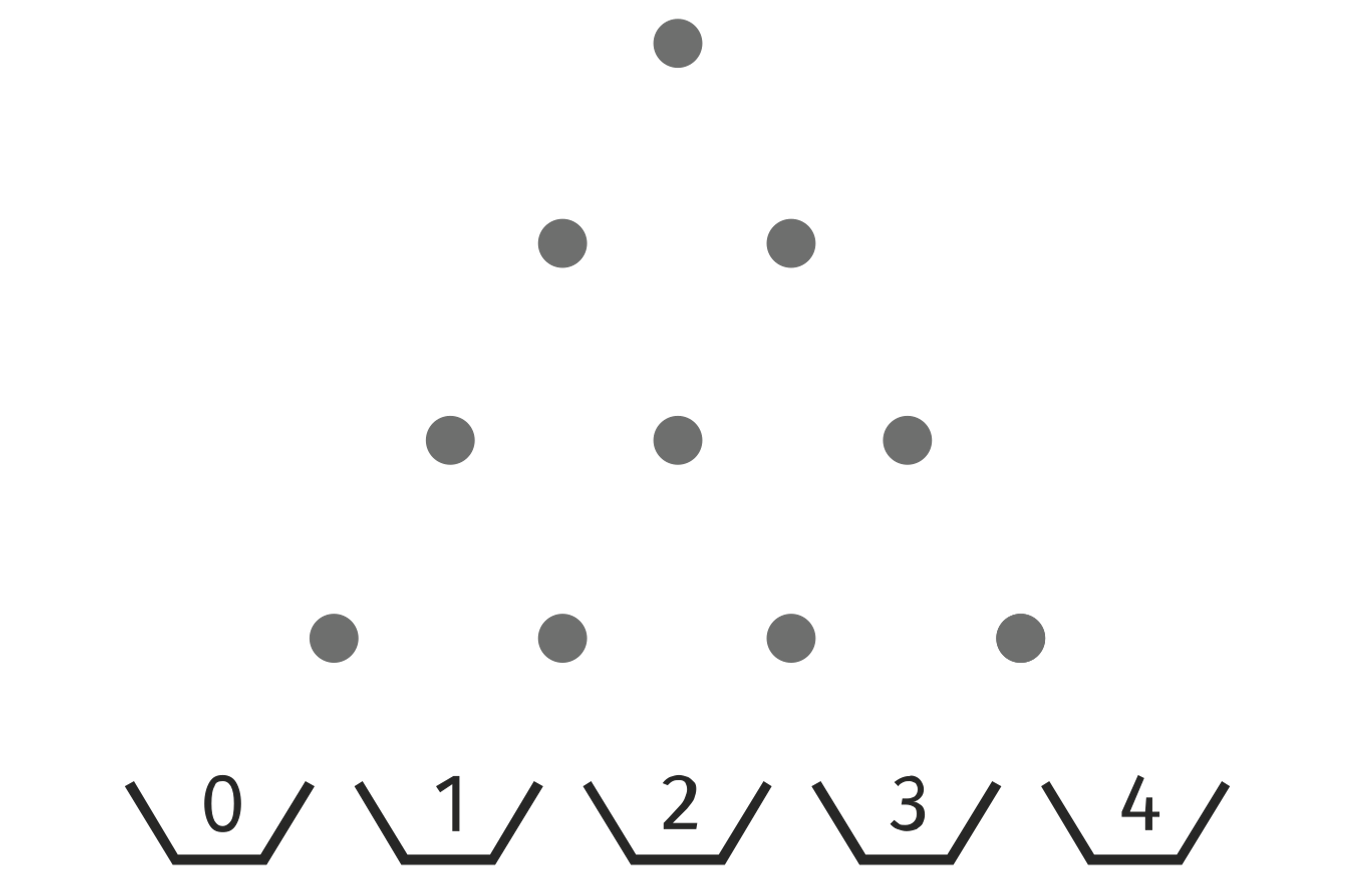
\includegraphics[width=6cm]{galton}
\end{minipage}
\begin{enumerate}
	\item 	Traduire cette situation par un arbre de probabilité.
	\item 	Soit $X$ la variable aléatoire qui, au lancer d'une bille associe le numéro de la case dans laquelle elle termine son parcours. Déterminer la loi de probabilité de $X$.
\end{enumerate}
%\vspace{0.5cm}

\exo{}
On lance un dé icosaédrique, dont les faces sont numérotées de 1 à 20, que l'on suppose bien équilibré. On marque :

	\begin{enumerate}[label=\textbullet]
		\item 	2 points si le nombre obtenu est pair ;
		\item 	3 points si le nombre obtenu est premier ;
		\item	5 points si le nombre obtenu est un multiple de 5 ;
		\item	7 points si le nombre obtenu est un carré parfait.	
	\end{enumerate}
Les points sont cumulables.\\
Soit $X$ la variable aléatoire qui associe au lancer du dé le nombre de points marqués par le joueur.
\begin{enumerate}
	\item 	Déterminer la loi de probabilité de $X$.
	\item 	En déduire $P(X\leqslant 5), P(3\leqslant X \leqslant7)$ et $P(X>7)$.	
\end{enumerate}

\subsection*{Espérance, variance et écart-type}

\exo{}
Dans chaque cas, calculer l'espérance, la variance et l'écart-type de la variable aléatoire $X$ dont on donne la loi de probabilité. Arrondir les résultat à $10^{-2}$ si nécessaire.
\begin{multicols}{2}
	\begin{enumerate}
		\item 	 $\quad$\\
		\begin{tabular}{|c|c|c|c|c|c|}
			\hline
			\cellcolor{UGLiOrange} $x_i$ & $-$4 & 1 & 3 & 7 & 12\\
			\hline
			\cellcolor{UGLiOrange} $P(X=x_i)$ & 0,15 & 0,4 & 0,3 & 0,05 & 0,1\\
			\hline
		\end{tabular}
	\vspace{2cm}
		\item 	$\quad$\\
		\begin{tabular}{|c|c|c|c|c|c|}
			\hline
			\cellcolor{UGLiOrange} $x_i$ & $-$5 & $-$2 & 0 & 1 & 4\\
			\hline
			\cellcolor{UGLiOrange} & & & & & \\
			 \cellcolor{UGLiOrange} $P(X=x_i)$ & $\dfrac{1}{12}$ & $\dfrac{1}{4}$ & $\dfrac{1}{6}$ & $\dfrac{1}{6}$ & $\dfrac{1}{3}$\\
			 \cellcolor{UGLiOrange} & & & & & \\
			\hline
		\end{tabular}
	\end{enumerate}
\end{multicols}
%\vspace{1cm}


\exo{}
Après avoir misé une certaine somme d'argent, un joueur lance un dé à 6 faces.\\
Il gagne 3 € s'il obtient un diviseur de 6.\\[0.5em]
Quel doit être le montant de la mise pour que le jeu soit équitable (c'est-à-dire pour que l'espérance de gain soit nulle) ?
%\vspace{1cm}


\exo{}
Un urne contient quatre boules rouges, trois boules jaunes, deux boules vertes et une boule bleue.\\
On tire au hasard une boule de l'urne et on note sa couleur.
\begin{enumerate}
	\item 	Déterminer la probabilité des événements suivants :\\
	R : « Tirer une boule rouge »\\
	J : « Tirer une boule jaune »\\
	V: « Tirer une boule verte »\\
	B: « Tirer une boule bleue »
	\item 	On gagne 10 points lorsqu'on tire une boule bleue, 5 pour une boule verte, 2 pour une jaune et 1 pour une rouge.\\
	On note $X$ la variable aléatoire qui associe à chaque tirage le nombre de points gagnés.
	\begin{enumalph}
		\item 	Déterminer la loi de probabilité de $X$.
		\item 	Déterminer p$(X\geq 3)$.
		\item	Calculer l'espérance, la variance et l'écart-type de $X$.
		\item	Interpréter l'espérance.
	\end{enumalph}
\end{enumerate}
%\vspace{0.5cm}


\exo{}
Trois jetons $A$, $B$ et $C$ sont placés dans cet ordre sur 3 cases numérotées 1, 2 et 3.\\
On prend les 3 jetons et on les replace au hasard sur les 3 cases.
\begin{enumerate}
	\item 	À l'aide d'un arbre, représenter les issues de cette expérience.
	\item 	$X$ est la variable aléatoire qui à chaque issue associe le nombre de jetons se retrouvant à leur place initiale.
	\begin{enumalph}
		\item 	Déterminer la loi de probabilité de $X$.
		\item 	Calculer $E(X)$.
	\end{enumalph}
\end{enumerate}
%\vspace{0.5cm}

\exo{}
La loi de probabilité d'une variable aléatoire $X$ est résumée dans le tableau suivant :
\begin{center}
	\begin{tabular}{|c|c|c|c|c|c|}
		\hline
		\cellcolor{UGLiOrange}\textbf{{$x_i$}} & 1 & 3 & 4 & 5 & 6\\
		\hline
		\cellcolor{UGLiOrange}{\boldmath $P(X=x_i)$} & 0,2 & 0,1 & 0,3 & 0,3 & 0,1\\
		\hline
	\end{tabular}
\end{center}
\begin{enumerate}
	\item 	Calculer l'espérance et la variance de $X$.
	\item 	Déterminer le réel $b$ tel que la variable aléatoire $Y=X+b$ ait une espérance nulle.
	\item 	Déterminer la valeur exacte du réel positif $a$ tel que la variable aléatoire $Z=aX$ ait une variance égale à $1$.\\
\end{enumerate}

\exo{}
Une enquête est réalisée par SMS. Lorsque l'abonné répond à l'enquête, il participe automatiquement à un tirage au sort et gagne $30$ min de 
communication une fois sur six, 20 min une fois sur trois et sinon 10 min.\\
$X$ est la variable aléatoire qui prend pour valeur le nombre de minutes gagnées.
\begin{enumerate}
	\item 	Calculer $E(X)$ et interpréter cette valeur.
	\item 	L'enquête est maintenant ciblée sur des adolescents. On remplace alors chaque minute gagnée par 5 SMS auxquels s'ajoutent 20 SMS pour 
	tous.\\
	$Y$ est la variable aléatoire qui prend pour valeur le nombre de SMS gagnés.\\
	- Exprimer $Y$ en fonction de $X$.\\
	- En déduire $E(Y)$.\\
\end{enumerate}
%\vspace{0.5cm}


\exo{}
Une étude statistique menée lors des entraînements de la saison montre que, sur une série de 5 tirs au but, Pierre marque 5 buts avec une 
probabilité de 0,2, 4 buts avec une probabilité de 0,5 et 3 avec une probabilité de 0,3.\\
Aujourd'hui, Pierre effectue deux séries de 5 tirs au but, on admet que les résultats de chaque séries sont indépendants.
\begin{enumerate}
	\item 	Construire un arbre pondéré modélisant cette expérience.
	\item 	$X$ est la variable aléatoire qui prend pour valeur le nombre total de buts.\\
	- Déterminer la loi de probabilité de $X$.\\
	- Calculer $E(X)$.\\
\end{enumerate}
%\vspace{0.5cm}


\exo{}
Une urne contient des jetons bleus, des jetons blancs et des jetons rouges.\\
10 \% des jetons sont bleus et il y a trois fois plus de jetons blancs que de jetons bleus.\\
Un joueur tire un jeton au hasard.
\begin{enumerate}[label=\textbullet]
	\item 	S'il est rouge, il remporte la mise de base ;
	\item 	S'il est blanc, il remporte le carré de la mise de base ;
	\item	S'il est bleu, il perd le cube de la mise de base.
\end{enumerate}
\begin{enumerate}
	\item 	On suppose que la mise de base est de 2 euros.
	\begin{enumalph}
		\item 	Soit $X$ la variable aléatoire qui donne le gain algébrique du joueur.\\
		Déterminer la loi de probabilité de X.
		\item 	Calculer le gain moyen que l'on peut espérer réaliser sur un grand nombre de tirages.
	\end{enumalph}
	\item 	On cherche à déterminer la valeur $g_0$	de la mise de base telle que le gain moyen réalisé sur un grand nombre de tirages soit maximal. Le résultat sera arrondi au centime d’euro. Soit $x$ la mise de base en euro.
	\begin{enumalph}
		\item 	Montrer que le problème posé revient à étudier les éventuels extremums de la fonction $f$ définie sur $\fio{0}{+\infty}$ par $\quad f(x)=-0,1x^3+0,3x^2+0,6x$.
		\item 	Déterminer la dérivée de la fonction $f$ sur l'intervalle $\fio{0}{+\infty}$.
		\item	En déduire le sens de variation de $f$ sur $\fio{0}{+\infty}$.
		\item	Conclure sur le problème posé.
	\end{enumalph}
\end{enumerate}




\end{document}
